\documentclass{article}
\usepackage{ctex}
\usepackage{color}
\usepackage{listings}
\usepackage{graphicx}
\usepackage{float}
\usepackage{subfig}
\usepackage{overpic}
\lstset{ %
basicstyle=\footnotesize,       % the size of the fonts that are used for the code
numbers=left,                   % where to put the line-numbers
numberstyle=\footnotesize,      % the size of the fonts that are used for the line-numbers
stepnumber=1,                   % the step between two line-numbers. If it is 1 each line will be numbered
numbersep=5pt,                  % how far the line-numbers are from the code
backgroundcolor=\color{white},  % choose the background color. You must add \usepackage{color}
showspaces=false,               % show spaces adding particular underscores
showstringspaces=false,         % underline spaces within strings
showtabs=false,                 % show tabs within strings adding particular underscores
frame=single,           % adds a frame around the code
tabsize=2,          % sets default tabsize to 2 spaces
captionpos=b,           % sets the caption-position to bottom
breaklines=true,        % sets automatic line breaking
breakatwhitespace=false,    % sets if automatic breaks should only happen at whitespace
}

\title{\heiti User Manual For Painkiller Injection System}
\author{%
  Panxin Tao, Runkang Yang, Zhekai Zhang\\
  SIST, ShanghaiTech University\\
  \texttt{taopx2022@shanghaitech.edu.cn}\\
  \texttt{yangrk2022@shanghaitech.edu.cn}\\
  \texttt{zhangzhk2022@shanghaitech.edu.cn}\\
}
\date{June 2024}
\begin{document}
\maketitle
\newpage
\section{Contents}
\subsection{System Introduction}
\subsubsection{Overview}
\subsubsection{Target Users}
\subsubsection{Running Guide}
\subsection{Interfaces}
\subsubsection{Structure}
\subsubsection{Physician Interface}
\subsubsection{Patient Interface}
\subsection{Issue Handling}
\subsection{Self-Testings}
\subsection{Notes}

\newpage
\section{System Introduction}
\subsection{Overview}
In medical practice, injections are often necessary for patient care, and the Painkiller Injection System provides two methods to meet various patient needs.
The first method is the baseline injection, which involves continuously injecting medication to maintain a stable level of pain relief. This method is suitable for patients requiring constant pain control, as it allows for a steady infusion of medication at a preset rate. Users can start and stop the baseline injection through the system and adjust the infusion rate as needed to ensure the patient receives the appropriate dosage.
The second method is the bolus injection, used when a patient experiences sudden, intense pain and requires immediate relief. This feature allows healthcare professionals to quickly administer a single dose of medication, providing rapid pain alleviation.
The system also allows for adjusting the bolus amount to cater to the patient's specific needs.

The Painkiller Injection System, built on Python, offers several essential functions, including starting and stopping baseline injections, administering bolus injections, and adjusting injection parameters. To ensure patient safety, the system imposes strict limits: no more than 1 mL per hour and 3 mL per 24 hours for combined baseline and bolus injections.
If these limits are about to be exceeded, the system will automatically halt all injections and alert the user, preventing overdose. The system's intelligent control, user-friendly interface, and customizable settings provide efficient and precise medication management, enabling healthcare professionals to deliver optimal pain relief to patients at all times.
\subsection{Target Users}
The target users of the Painkiller Injection System are divided into two distinct groups: patients and physicians, each with a tailored interface to meet their specific needs.

For patients, the interface is designed to be user-friendly and intuitive, allowing them to request a bolus injection when experiencing acute pain. This functionality ensures that the requested bolus does not exceed the established safety limits, providing patients with a secure and reliable means to manage their pain. The patient interface prioritizes ease of use and accessibility, enabling patients to interact with the system with minimal effort and maximum confidence.

For physicians, the interface is equipped with a comprehensive set of features to facilitate effective pain management. Physicians can easily switch the baseline injection on and off, allowing for continuous medication delivery or its cessation as needed. Additionally, they have the capability to adjust the rates of both baseline and bolus injections, tailoring the medication regimen to the specific requirements of each patient. This advanced interface provides healthcare professionals with the tools necessary to monitor and control pain relief precisely, ensuring optimal care and patient safety. By offering these specialized interfaces, the Painkiller Injection System caters to the unique roles and responsibilities of both patients and physicians.
\subsection{Running Guide}
Firstly, make sure that you have installed Python. Make sure your operation system and Python satisfy:

Operating System: Windows 10 or higher, MacOS 10.14 or higher, Linux Ubuntu 18.04 or higher.

Then, install the PyQt5 library using the codes in Command Prompt of Windows or Terminal of MacOS or Linux:
\begin{lstlisting}
pip install PyQt5
\end{lstlisting}
Enter the \lstinline!src! package, which is the location of \lstinline!main.py!.
Finally, input the command below:
\begin{lstlisting}
python3 main.py
\end{lstlisting}
\section{Interfaces}
\subsection{Structure}
It's divided into the "Physician Interface" and the "Patient Interface". The details are as below:
\subsection{Physician Interface}
Here's the entire interface:
\begin{figure}[htbp]
  \centering
  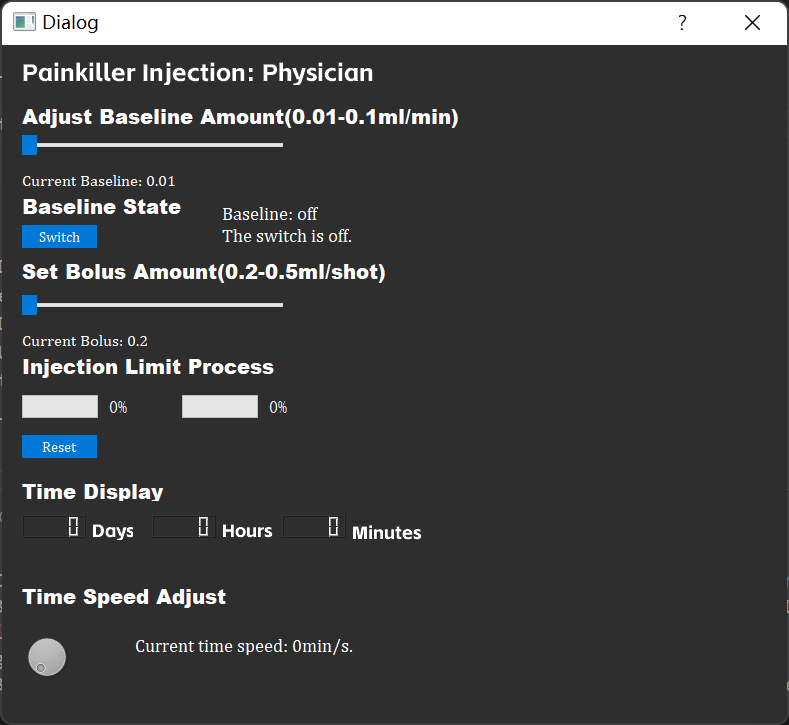
\includegraphics{img/physician_ui.png}
  \caption{Physician Interface}
\end{figure}

1. The upmost scrollbar is used to adjust the baseline amount, which ranges from $\textbf{0.01ml/min}$ to $\textbf{0.1ml/min}$.

2. The line beside it responses to the baseline adjustment, which displays the current baseline amount. It will still display a number between 0.01 and 0.1 when baseline is not being injected.

3. The switch button can also be pressed at any time, representing a valid switch change. If the switch is off, the baseline is not injecting. Else, if will depend on whether or not it's to exceed the restrictions.

4. There are two lines beside the switch. One shows whether the switch is on or off, while the other one displays whether the baseline is being injected or not.

5. The second scrollbar is used to set bolus amount. The line below is also similar to the former one.

6. The two process bars represent the ratio of the injection amount during the last one hour(day) and the upper bound restriction of injection amount one hour(day). It's updated continuously.

7. The reset button can be pressed at any time. When pressed, all former records of injections will be cleared.

8. The time display area displays the time(measured by the normal time pass multiplies the time speed) since the opening of the system. The format is $\textbf{day+hour+minute}$.

9. The time speed adjust dial is used to adjust the time speed in the system. When it's $\textbf{0min/s}$, for instance, it means the system time is paused. When it's $\textbf{1min/s}$, 1 second in real life represents 1 minute in the system.
\subsection{Patient Interface}
Here's the entire interface:
\begin{figure}[htbp]
  \centering
  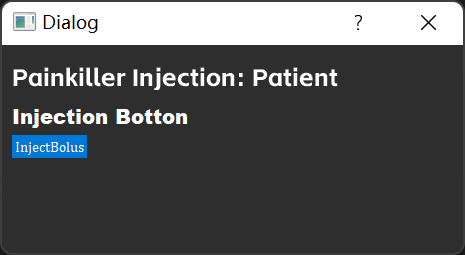
\includegraphics{img/patient_ui.png}
  \caption{Patient Interface}
\end{figure}

1. The InjectBolus button can be pressed at any time. However, the system gives different responses. If it's to exceed the restrictions, the injection fails and there will be a popup informing you of the failure. On the contrary, if the injection succeeds, it'll be recorded and a popup will emerge, offering you the detailed information as well.
\section{Issue Handling and Notes}
1. You can only adjust baseline when the switch is off. When the switch is on, the scrollbar enable is set to false.

2. The bolus scrollbar can be adjusted at any time.

3. The time display will not be reset when the $\textbf{Reset}$ button is clicked.

4. The FPS will change with the time speed to ensure each one update corresponds to one system minute.
\end{document}
